\section{Preliminaries}
\subsection{Graph databases}
%%

References:
\begin{itemize}
    \item PG: \cite{PG-angles2017foundations, PG-angles2018propertyGraphDatabaseModel, PG-Graphs-at-a-time-GraphQL-QueryLanguage, PG-exampleUsageSimeonovski}
    \item Graph Databases: \textcolor{blue}{\cite{GDB-angles2008survey, GDB-kumar2015graph}}
\end{itemize}
\subsection{Graph fraud patterns}
xxxxx
\fmc{Aqui ponemos referencias / describimos los fraudes bancarios que existen... informe SEPA? - o solo en la introducción?}
%%
\subsubsection*{Graph Database Model: Property Graph}

Informally, a property graph is a directed labeled multigraph with the special characteristic that each node or edge could maintain a set (possibly empty) of property-value pairs \cite{angles2018propertyGraphDatabaseModel}. In this graph, a node represents an entity, an edge a relationship between entities, and a property represents a specific feature of an entity or relationship. 
A more formally  (as defined in \cite{PG-exampleUsageSimeonovski}):

\begin{definition}
A property graph $G=(V,E, \lambda, \mu)$ is a directed labeled multigraph where $V$ is a set of nodes, $E \subseteq (V \times V)$ is a set of edges, $\lambda: V \cup E \rightarrow \Sigma$ is a function that labels nodes and edges with symbols of the alphabet $\Sigma$, and $\mu: (V \cup E) \times K \rightarrow S$ is a function that associates key-value properties, e.g., $(k,s)$ where $k \in K$ is the key and $s \in S$ is the string value, to nodes and edges.  
\end{definition}

\ad{Aqui estaría bien un ejemplo pequeño, dos nodos con un arco entre ellos y varias posibles propiedades, para que quede bien claro lo que es.}

\ad{añadir algo como lo siguiente: In the Graph Database community there several popular models of property graphs. Maybe the two most famous and used ones are \ldots 
los dos màs famosos con cita a algun sitio que diga que son los más famosos}

\ad{Muy importante: antes de explicar detalles específicos de Neo4j hay que explicar todo lo que es genérico de los property graphs y ponerlo aquí, fuera de la subsección de Neo4j}

\subsubsection*{Graph Database System: Neo4j}

Graph Databases: \textcolor{blue}{\cite{GDB-angles2008survey, GDB-kumar2015graph}}
% TODO: 
% - Poner definición 
% - Decir cuál elegimos: Neo4j y por qué

A graph database system is a system specifically designed for managing graph-like data following the basic principles of databases systems. 

%%
%%
\subsection{Dynamic Pipeline Paradigm}\label{DPP}

\textcolor{gray}{To explain:
\begin{itemize}
    \item PP (Pipeline Parallelism) computational model. The definition
    \item DP stages y un poco que hace cada stage
    \item Problemas que ya se han resuelto con este paradigma. Referenciar.
\end{itemize}
}

\fmc{Definición - Tomada de TFM Dani y J Pablo... completar mas?}

\ad{Yo creo que puedes citar ambas tesis y también el paper de Edelmira y explicar lo que es pero no hace falta que entres en demasiado detalle general, eso sí, los detalles de cómo lo usas para lo tuyo sí deben estar completos.}
In the context of Stream Processing, many data driven frameworks have emerged to address the management of continuous data streams. Dynamic data processing, characterized by the adaptive and responsive manipulation of large datasets in real time, and incremental generation of results, represent pivotal approaches.\\

One such model for Stream Processing is the Dynamic Pipeline Paradigm ($\mathsf{DPP}$) \cite{DP-pasarella2024computational}. The $\mathsf{DPP}$ is a PP (Pipeline Parallelism) data driven computational model that operates as a one-dimensional, unidirectional chain of stages connected by means of data channels. Essentially, the paradigm establishes a computational model rooted in the deployment of a linear pipeline consisting of a chain of stages structure called Dynamic Pipeline ($\mathsf{DP}$). It stretches and
shrinks depending on the spawning and the lifetime of its stages, respectively. Stages are processes that execute tasks concurrently/in-parallel.\\

\begin{figure}[H]
  \centering
  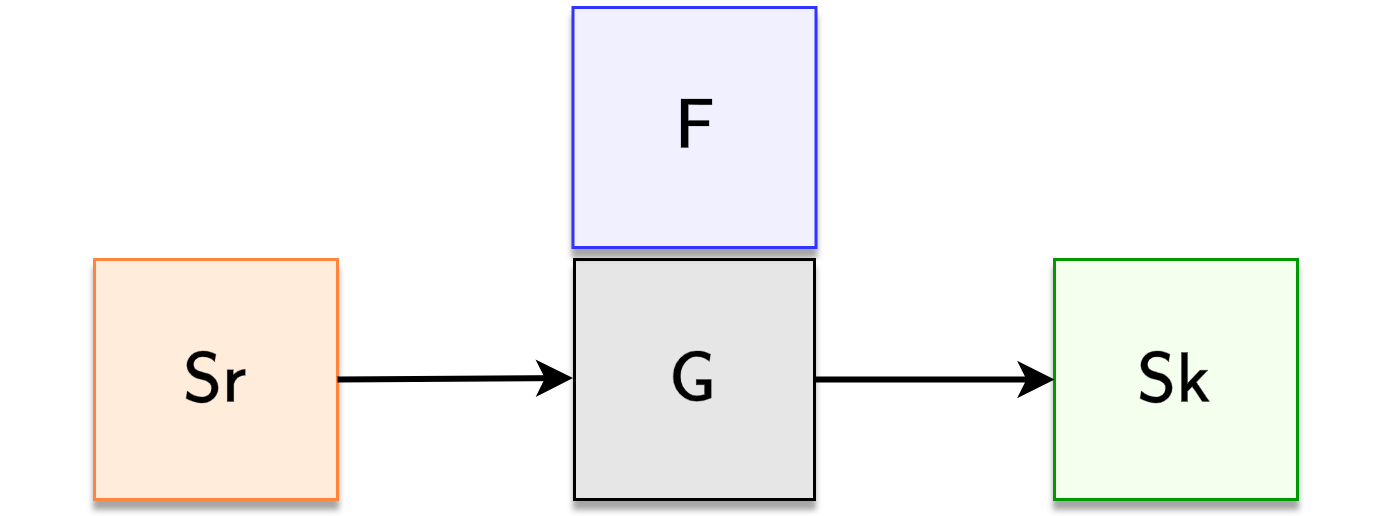
\includegraphics[scale = 0.7]{images/3-Engine/DP-Stages-1.png}
  \caption{Initial configuration of a Dynamic Pipeline. An initial $\mathsf{DP}$ consists of three stages: \emph{Source} ($\mathsf{Sr}$), \emph{Generator} ($\mathsf{G}$) and \emph{Sink} ($\mathsf{Sk}$). Above the  \emph{Generator} ($\mathsf{G}$) the \emph{Filter} ($\mathsf{F}$) parameter. The stages are connected through its channels, represented with the black right arrows.}
  \label{img:DP-Stages-1}
\end{figure}

These stages can be of four different types: \emph{Source} ($\mathsf{Sr}$), \emph{Filter} ($\mathsf{F}$), \emph{Generator} ($\mathsf{G}$) and \emph{Sink} ($\mathsf{Sk}$). \emph{Source} stage are the responsible of obtaining the input data stream and feeding it into the pipeline. \emph{Filter} stages maintain a state and process the incoming data processing it accordingly and/or passing it again to the pipeline. \emph{Generator} stage is in charge of spawning new \emph{Filter} stages when needed based on the incoming data, providing the \textit{dynamic} behavior to the model. Finally, \emph{Sink} stage receives the results, processing and acting on them as needed.
Figure \ref{img:DP-Stages-1} represents the initial configuration of a $\mathsf{DP}$ and Figure \ref{img:DP-Stages-2} depicts the stages of the $\mathsf{DP}$ after a possible evolution, where the \emph{Generator} has created two \emph{Filter} stage instances.\\

\begin{figure}[H]
  \centering
  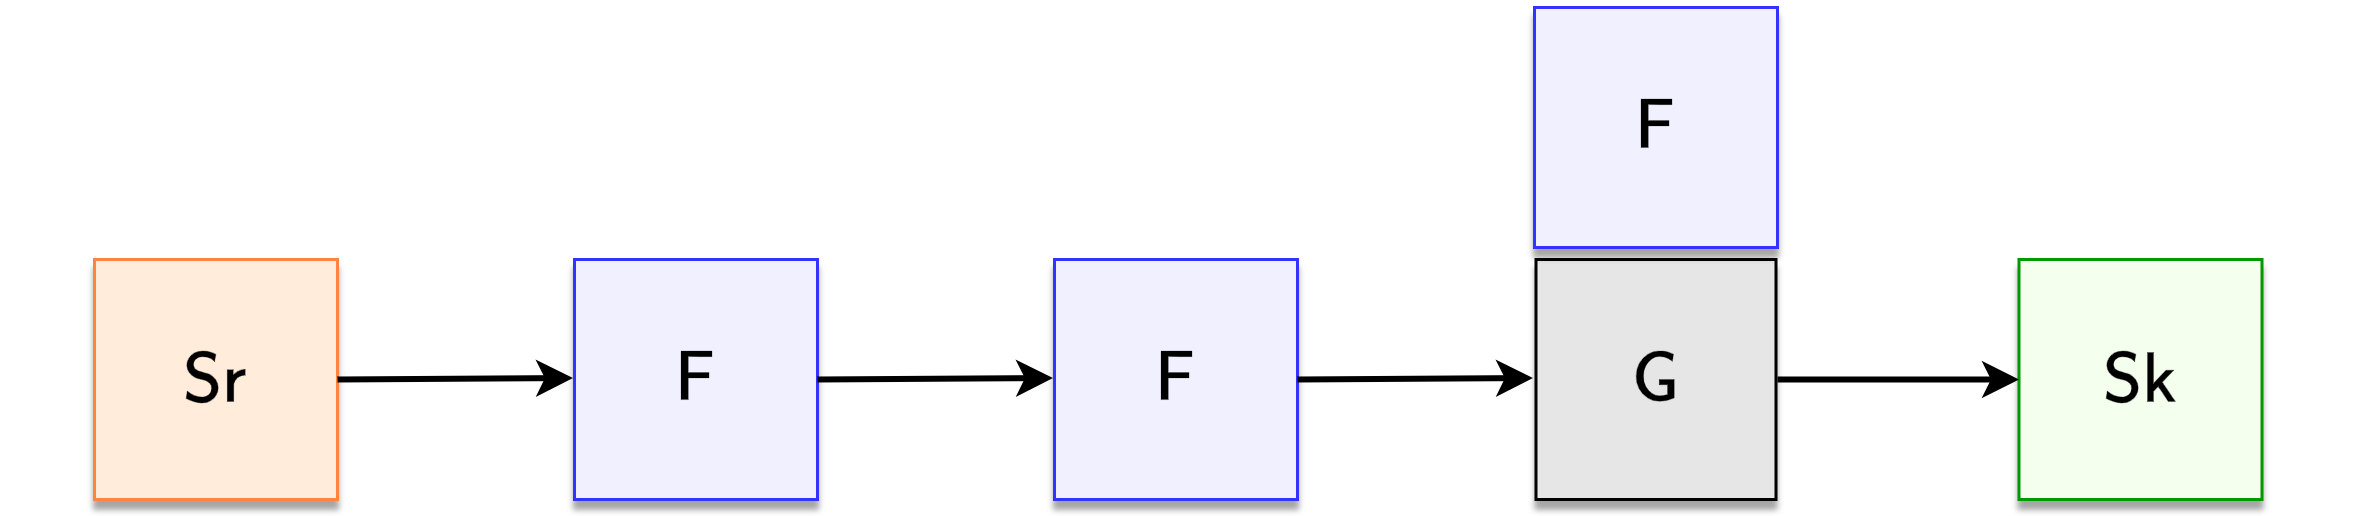
\includegraphics[scale = 0.7]{images/3-Engine/DP-Stages-2.png}
  \caption{Evolution of a $\mathsf{DP}$. After the creation of two \emph{Filter} $\mathsf{F}$ stage instances of the \emph{Filter} parameter (above the $\mathsf{G}$ stage) by the \emph{Generator} $\mathsf{G}$ stage.}
  \label{img:DP-Stages-2}
\end{figure}

The $\mathsf{DPP}$ has been used to model many different problems. In \cite{DP-bitriangles2021} they successfully solved the problem of progressively identify and enumerate bitriangles (i.e. a specific graph pattern) in bipartite evolving graphs. In \cite{DP-Lugosi_Enes_2019} $\mathsf{DPP}$ is used to model the problem of multidimensional range queries, that is, selection queries on objects in a k-dimensional space. Finally, in \cite{DP-Benedi_Garcia_2024} they solve the problem of computing and maintaining the minimum spanning tree of dynamic graphs.\\

In our case, we envision the architecture of our continuous query engine to detect anomalous ATM transactions under the $\mathsf{DPP}$, where the continuous input data stream is the stream of the bank ATM transactions, and we track the activity of a Card on a certain \emph{Filter} stage. Details on how the modeling of our problem with the $\mathsf{DPP}$ can be found in \ref{ContinuousQueryEngine}.
%%
%%
\subsection{Diefficiency metrics}

\fmc{Las tengo en \ref{exps:evaluation-metrics}, aquí hacer referencia y citar las de diefficiency del artículo y la herramienta utilizada, luego ya en el apartado de Experiments ponerlas todas (+ las adicionales añadidas, como interactions/s o el response time)}





